基础模型提供可复用的表示，但将其适配到下游应用往往需要不同机构或设备持有的数据。联邦学习使这些数据持有方无须汇集原始样本，就能优化共享模型~\cite{mcmahan2017communication,kairouz2021advances}。对于内存、计算和通信能力有限的客户端，完整参数更新仍然代价高昂。低秩适配（LoRA）保持预训练主干固定，用紧凑的可训练因子表示更新，从而降低这一负担~\cite{hu2022lora}。因此，联邦 LoRA 使协同适配更易实施，但仍需决定每个客户端应利用其可用资源更新哪些适配器参数。

适配器大小本身不能决定训练是否可行。冻结主干、优化器状态以及反向传播时保留的中间激活也需要内存。降低秩会缩小适配器相关状态，却不一定缩短到可训练位置的反向传播路径。Fed-HeLLo 指出这一区别，并报告在激活占主导的设置中，降低秩带来的总内存节省有限~\cite{zhang2025fedhello}。因此，选择可训练位置是秩调整的补充：它改变更新发生的位置，并且在部分适配器执行方式下改变必须保留的激活依赖。我们在固定秩下研究这一位置决策，将目标选择与选中适配器内部的容量分配区分开来。

Transformer 块包含查询、键、值和前馈变换等不同的目标投影。每个投影都可以接收自己的 LoRA 更新。已有位置研究和重要性感知秩分配表明，不同矩阵或层的适配价值不必相同~\cite{hu2022lora,fm_adalora2023}。然而，层级分配将块内候选投影绑定为同一个决策。在有限预算下，选择一个有用的投影可能因此必须同时给同块的其他投影分配容量，并排除别处有用的目标。这引出一个比“不同位置是否重要”更具体的问题：在重要性准则和参数预算固定时，解除完整层绑定能否改善所选的适配配置？

为考察这一问题，我们在 CIFAR100/ViT-base 上比较独立矩阵选择与完整层分配。矩阵级分配从 12 个 Transformer 块中选择 12 个 Q/K/V 目标矩阵；层级分配选择四个块中的全部三个投影。两者均使用秩 8，且可训练参数数量相同。在每一种评分来源下，它们在相同解析式资源限制内最大化同一个画像效用。我们分别评估本地评分与服务器代理评分，涵盖 IID 数据及浓度参数为 $1.0$ 和 $0.1$ 的 Dirichlet 划分。配对配置从初始化或共同预热后的同一适配器出发，进行 20 步本地训练。在前向模型中保留但冻结未选适配器，以隔离可训练子集的影响。第~\ref{sec:fm-granularity-study} 节详述协议。

图~\ref{fig:fm-motivation} 报告矩阵级减去层级的留出验证损失下降量差值。全部 12 个“划分--检查点--评分来源”设置的均值均为正；36 个种子内配对均值中有 35 个为正，每个种子内先对五个客户端求平均。本地和服务器代理重要性评分下均观察到这种改进。这一观察支持独立目标选择作为超越完整层分配的有用适配维度，而不是将收益归因于某一种评分来源。测得的结果是在固定参数预算下的短期损失下降。

\begin{figure*}[!t]
  \centering
  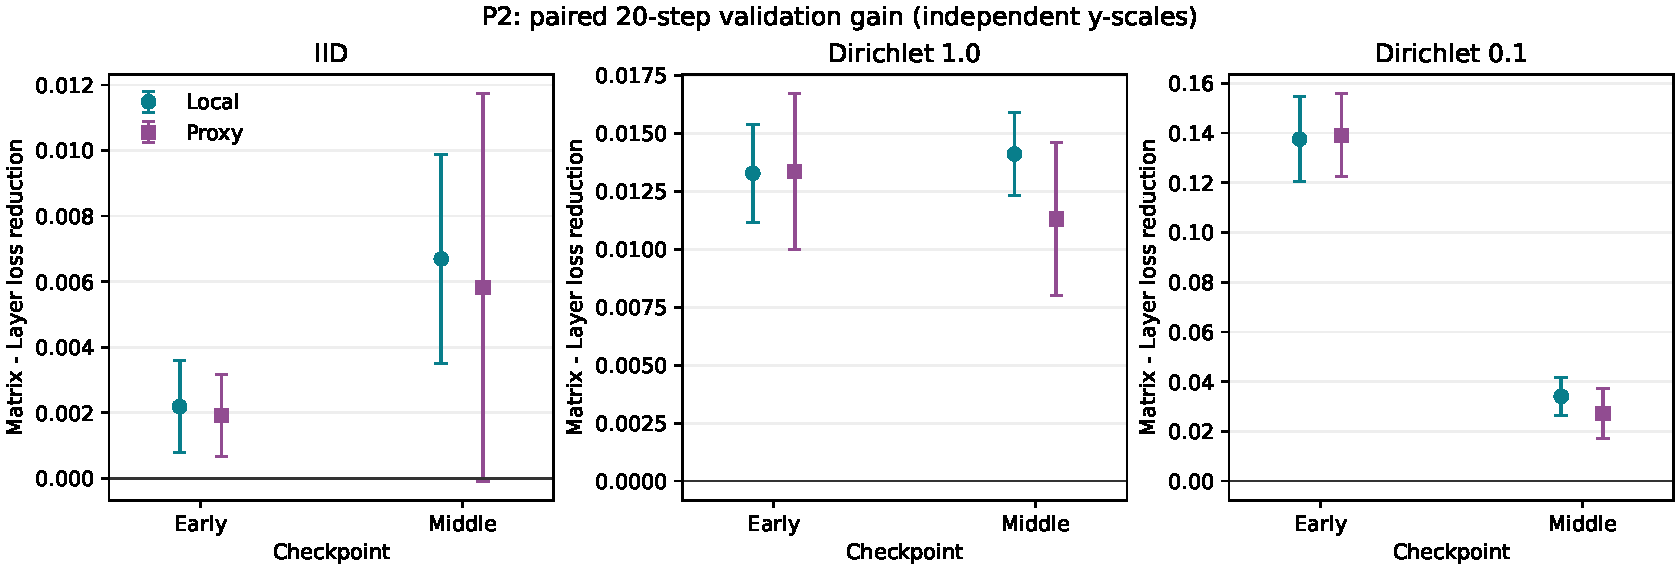
\includegraphics[width=.98\textwidth]{figures/fig1_p2_granularity.pdf}
  \caption{CIFAR100/ViT-base 上矩阵级选择相对于完整层分配的配对短期改进。纵轴为 20 步后留出验证损失下降量的矩阵级减层级差值；正值表示矩阵级选择更优。两类配置均包含 12 个秩为 8 的目标，且每组对比使用相同评分来源。在 Local 和 Proxy 评分下分别评估初始化及独立预热后的检查点。均值先在每个种子内对五个客户端求平均；误差棒表示三个种子间的样本标准差。各面板使用不同的纵轴刻度。}
  \label{fig:fm-motivation}
\end{figure*}

利用这种灵活性，需要在投入训练预算之前评估候选更新。基于梯度和 Fisher 的准则提供了确定可训练参数及 LoRA 层优先级的已有方法~\cite{fm_fish2021,zhang2025fedhello}。这些优先级同时依赖当前模型及评估其损失所用的数据。在联邦系统中，每个客户端已持有定义其本地目标的数据。评估该目标可以提供客户端相关的判断，而不要求服务器另持有画像数据集。Fed-pilot 也将本地及汇总的重要性信息纳入 LoRA 分配~\cite{fm_fedpilot2025}；本文的重点是在块内开放单独的投影选择，并在耦合资源约束下协调这些选择。本地画像是评估机制，动机实验则隔离选择粒度的价值。

但是，高评分子集只有能够训练才有用。内存可行性不仅取决于所选目标的数量，还取决于其位置；客户端计算能力与带宽决定配置能否满足轮次截止时间。即使各项选择单独可行，一起执行时也可能超出共享轮次预算。因此，设计有两个相互关联的要求：在目标矩阵粒度估计更新优先级，并将其转化为可在同一训练轮次协调的客户端可行配置。仅有排序无法解决第二个要求。

为满足这些要求，本文提出 FedMATRIX-LoRA，一种面向资源受限联邦微调的客户端感知矩阵级适配框架。在画像刷新时，每个客户端在当前全局适配器下，使用一个本地小批次评估候选投影的 LoRA 因子。所得评分指导不同矩阵等价成本下的配置，同时满足本地内存和时延限制。服务器在共享预算和同步时延目标下选择客户端配置。客户端训练分配的因子，再按矩阵聚合以更新共享的全局适配器。本地证据指示偏好的目标；资源感知分配决定哪些提议的更新可以共同执行。

本文贡献包括三点：
\begin{itemize}
\item 我们建立面向资源受限联邦微调的重要性引导目标矩阵选择模型，使 Transformer 块内的投影可以独立选择。参数预算匹配的受控研究，在本地与服务器代理两种评分下，以实际短期适配收益说明这一粒度的动机。
\item 我们提出 FedMATRIX-LoRA，将本地矩阵画像、资源可行配置生成、共享预算协调和按矩阵聚合连接起来。客户端可更新不同目标子集，同时对共同的全局适配器作出贡献。
\item 我们给出选择性聚合的条件性平稳性分析，并在图像分类、语言理解和对话摘要任务上评估框架。受控评分和消融研究将各机制与完整系统的性能分别考察。
\end{itemize}

第~\ref{Sec.relatedworks} 节将本文与已有工作比较。第~\ref{sec.model} 节定义系统模型和分配问题。第~\ref{Sec.alg} 节介绍框架及其分析，第~\ref{Sec.evaluation} 节报告评估。第~\ref{Sec.conclusion} 节总结全文。
